\documentclass[tikz,border=3pt]{standalone}
\usepackage[T1]{fontenc}
\usepackage{mathptmx}
\usepackage{tikz,pgfplots}
\usetikzlibrary{arrows.meta,positioning,calc,fit,backgrounds,shapes.geometric}
\pgfplotsset{compat=1.18}
\definecolor{forest}{HTML}{346E57}
\definecolor{sage}{HTML}{E8EFEA}
\definecolor{clay}{HTML}{AC653F}
\definecolor{sand}{HTML}{F4EAE2}
\definecolor{ink}{HTML}{252525}
\definecolor{light}{HTML}{F5F5F3}
\definecolor{gridgray}{HTML}{D8DAD6}
\tikzset{box/.style={draw=ink!70,line width=.5pt,rectangle,rounded corners=1pt,fill=white,align=center,font=\fontsize{11}{12}\selectfont,inner sep=6pt}, flow/.style={-{Latex[length=2.4mm]},line width=.7pt,draw=ink!80}, data/.style={flow,densely dashed,draw=forest}, label/.style={font=\fontsize{10}{11}\selectfont,fill=white,inner sep=2pt,align=center}}
\hyphenpenalty=10000\exhyphenpenalty=10000\begin{document}
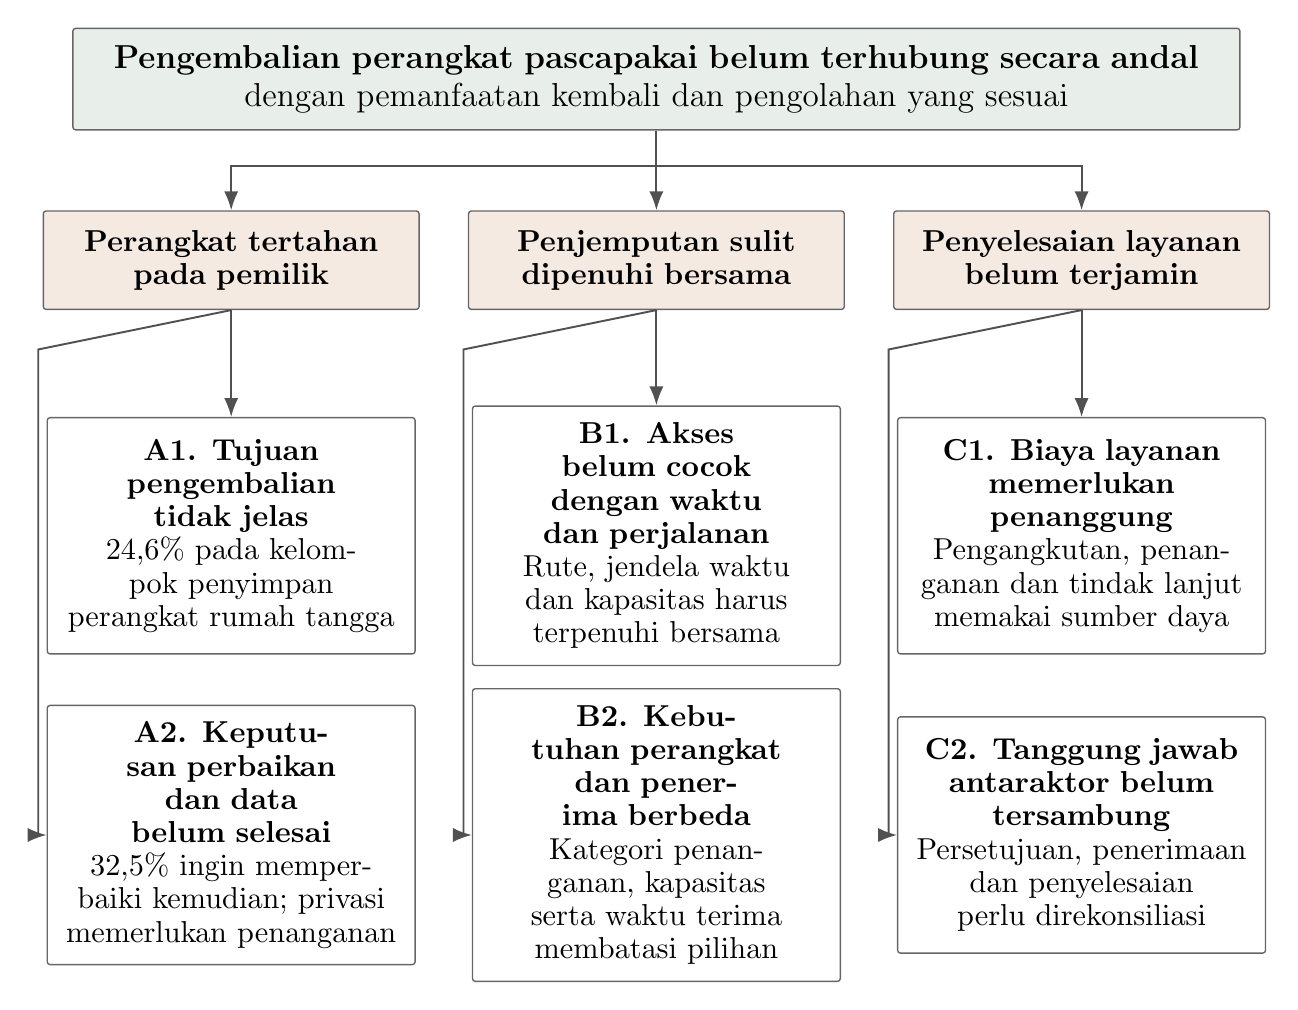
\begin{tikzpicture}[x=1cm,y=1cm]
\node[box,text width=14.4cm,fill=sage,font=\fontsize{12}{14}\selectfont] (problem) at (7.9,11.6) {\textbf{Pengembalian perangkat pascapakai belum terhubung secara andal}\\dengan pemanfaatan kembali dan pengolahan yang sesuai};
\foreach \x/\id/\text in {2.5/A/{Perangkat tertahan\\pada pemilik},7.9/B/{Penjemputan sulit\\dipenuhi bersama},13.3/C/{Penyelesaian layanan\\belum terjamin}} {
\node[box,text width=4.35cm,fill=sand,minimum height=1.25cm] (\id) at (\x,9.3) {\textbf{\text}};
\draw[flow] (problem.south)--++(0,-.45)-|(\id.north);
}
\node[box,text width=4.25cm,minimum height=3cm] (A1) at (2.5,5.8) {\textbf{A1. Tujuan pengembalian\\tidak jelas}\\24,6\% pada kelompok penyimpan perangkat rumah tangga};
\node[box,text width=4.25cm,minimum height=3cm] (A2) at (2.5,2.0) {\textbf{A2. Keputusan perbaikan\\dan data belum selesai}\\32,5\% ingin memperbaiki kemudian; privasi memerlukan penanganan};
\node[box,text width=4.25cm,minimum height=3cm] (B1) at (7.9,5.8) {\textbf{B1. Akses belum cocok\\dengan waktu dan perjalanan}\\Rute, jendela waktu dan kapasitas harus terpenuhi bersama};
\node[box,text width=4.25cm,minimum height=3cm] (B2) at (7.9,2.0) {\textbf{B2. Kebutuhan perangkat\\dan penerima berbeda}\\Kategori penanganan, kapasitas serta waktu terima membatasi pilihan};
\node[box,text width=4.25cm,minimum height=3cm] (C1) at (13.3,5.8) {\textbf{C1. Biaya layanan\\memerlukan penanggung}\\Pengangkutan, penanganan dan tindak lanjut memakai sumber daya};
\node[box,text width=4.25cm,minimum height=3cm] (C2) at (13.3,2.0) {\textbf{C2. Tanggung jawab\\antaraktor belum tersambung}\\Persetujuan, penerimaan dan penyelesaian perlu direkonsiliasi};
\foreach \id in {A,B,C}{\draw[flow](\id.south)--++(0,-.5)-|(\id1.north);\draw[flow](\id.south)--++(-2.45,-.5)|-(\id2.west);}
\end{tikzpicture}
\end{document}
